\documentclass{beamer}

\usepackage[utf8]{inputenc}
\usepackage{color, xcolor}

\usepackage{multicol}
\usepackage{fancyhdr}
\usepackage{listings}
\usepackage{graphicx, subfig}
\usepackage{float}
\usepackage{enumerate}

\usepackage{amsfonts}
\usepackage{eucal}
\usepackage{amsmath}
\usepackage{amssymb}
\usepackage{gensymb}
\usepackage{amsthm}
\usepackage{makecell}
\usepackage[ruled]{algorithm2e}
\usepackage{tikz}
\usetikzlibrary{positioning}

\usepackage[backend=bibtex,style=authoryear]{biblatex}
\bibliography{reference.bib}
\setbeamerfont{footnote}{size=\tiny}
\renewcommand{\thefootnote}{[\arabic{footnote}]}

\title{Project Report}
\author{Team \#12}
\institute{
  \parbox{0.2\textwidth}{
    \centering WANG Zeyu
    \vspace{.25cm}
  }
  \parbox{0.2\textwidth}{
    \centering YANG Xirui
    \vspace{.25cm}
  }
  \parbox{0.2\textwidth}{
    \centering Wu Tianxiao
    \vspace{.25cm}
  }
}
\date{\today}

\usetheme{Madrid}
\usecolortheme{default}
\setbeamertemplate{navigation symbols}{}

\setbeamertemplate{footline}
{
  \leavevmode%
  \hbox{%
  \begin{beamercolorbox}[wd=0.3\paperwidth,ht=2.25ex,dp=1ex,center]{author in head/foot}%
    \usebeamerfont{author in head/foot}\insertshortauthor
  \end{beamercolorbox}%
  \begin{beamercolorbox}[wd=.4\paperwidth,ht=2.25ex,dp=1ex,center]{title in head/foot}%
    \usebeamerfont{title in head/foot}\insertsection
  \end{beamercolorbox}%
  \begin{beamercolorbox}[wd=0.3\paperwidth,ht=2.25ex,dp=1ex,center]{date in head/foot}%
    \usebeamerfont{date in head/foot}\insertshortdate{}\hspace*{2em}
    \insertframenumber{} / \inserttotalframenumber\hspace*{2ex}
  \end{beamercolorbox}}%
  \vskip0pt%
}

\usefonttheme[onlymath]{serif}

\begin{document}

\section*{Cover}
\frame{\titlepage}

\section*{Contents}
\begin{frame}{Contents}
  \tableofcontents
\end{frame}

\section{Problem definition}

\begin{frame}{Problem definition}

  \begin{itemize}
    \item \textbf{Task 1}: Train models based on $10$ features, including academic metrics, aptitude scores, and soft skill ratings, to predicting whether a student will be successfully placed in a job. \vspace{.25cm}
    \item \textbf{Task 2}: Train models based on $18$ anonymity features and labeled with $5$ classes, then predict the labels based on the training set. \vspace{.25cm}
    \item \textbf{Task 3}: Train models based on $28$ anonymity numerical with the transaction amount, to indicate whether it is a fraudulent transaction or a legitimate transaction. \vspace{.25cm}
  \end{itemize}

\end{frame}

\section{Method}

\subsection{Data Prepare}

\begin{frame}{Correlation coefficient \footfullcite{abdi2007kendall} \footfullcite{hauke2011comparison}}

  \begin{itemize}
    \item \textbf{Pearson correlation coefficient}: Measures linear correlation between two sets of data; \vspace{.25cm}
    \item \textbf{Kendall correlation coefficient}: Measures the rank correlation by counting the concordant pairs; \vspace{.25cm}
    \item \textbf{Spearman correlation coefficient}: Measures the rank correlation based on the Pearson correlation coefficient; \vspace{.25cm}
  \end{itemize}

\end{frame}

\begin{frame}{$k$-nearest neighbors imputer \footfullcite{troyanskaya2001missing} \footfullcite{juna2022water}}

  The $k$-nearest neighbors imputer estimating the missing values using the $k$ nearest neighbors which: \vspace{.25cm}

  \begin{itemize}
    \item Works with both numerical and categorical data; \vspace{.25cm}
    \item Don't need any assumption about the data distribution; \vspace{.25cm}
    \item robust in many applications. \vspace{.25cm}
  \end{itemize}

\end{frame}

\begin{frame}{Dimension raising}

  Given the scalar data $x_i$ and a given degree $d$, we compute the new data as \vspace{.25cm}

  $$
    (x_i, x_i^2, \dots, x_i^d).
  $$ \vspace{.25cm}

  Combination of differnet features are also used in dimansion raising, e.g. given scalar $x_i$ and $y_i$, another kind of new data is computed as \vspace{.25cm}

  $$
    (x_i, y_i, x_i y_i).
  $$ \vspace{.25cm}

\end{frame}

\begin{frame}{Dimension raising}

  \begin{figure}[H]
    \centering
    \includegraphics[width=0.4\textwidth]{./figure/Sample-Raising-1.jpg}
    \includegraphics[width=0.4\textwidth]{./figure/Sample-Raising-2.jpg}
    \caption{Example for dimension raising. The left shows that origin data, where the data is not linearly separable, while the right shows the data after dimension raising, where the $y_2$ is easy to be separated by a line.}
  \end{figure}

\end{frame}

\subsection{Data Analysis}

\begin{frame}{Data Analysis}

  \begin{itemize}
    \item \textbf{The logistic regression} \footfullcite{walker1967estimation} \footfullcite{pohar2004comparison} is a widely used linear classification model, which gives a probability value ranging between $0$ and $1$. \vspace{.25cm}
    \item \textbf{The decision tree} \footfullcite{utgoff1989incremental} \footfullcite{kotsiantis2013decision} is a supervised learning method used for classification which predict the label with piecewise constant approximation.
    \item \textbf{The multilayer perceptron (MLP)} \footfullcite{rosenblatt1958perceptron} \footfullcite{rumelhart1986learning} is a basic kind of neural network which learns a function $f: \mathbb{R}^n \mapsto \mathbb{R}^m$ to approximate the input and output, with the ability of hierarchical feature extraction.
  \end{itemize}

\end{frame}

\section{Solution}

\subsection{Solution - Task 1}

\begin{frame}{Task 1 - Overview}

  \begin{figure}[H]
    \centering
    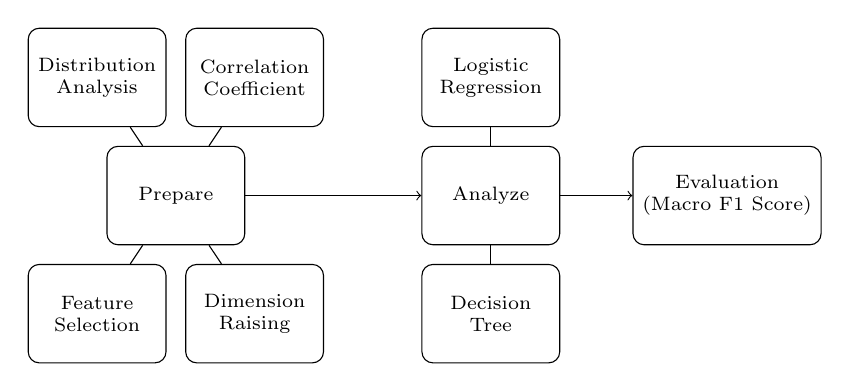
\begin{tikzpicture}[minimum width=1.75cm, minimum height=1.25cm, font=\scriptsize]
      \node[draw, align=center, rounded corners]  (P)   at ( 0,  0.0)    {Prepare};
      \node[draw, align=center, rounded corners]  (D)   at (-1,  1.5)    {Distribution \\ Analysis};
      \node[draw, align=center, rounded corners]  (C)   at ( 1,  1.5)    {Correlation \\ Coefficient};
      \node[draw, align=center, rounded corners]  (F)   at (-1, -1.5)    {Feature \\ Selection};
      \node[draw, align=center, rounded corners]  (R)   at ( 1, -1.5)    {Dimension \\ Raising};

      \node[draw, align=center, rounded corners]  (M)   at ( 4,  0.0)    {Analyze};
      \node[draw, align=center, rounded corners]  (LR)  at ( 4,  1.5)    {Logistic \\ Regression};
      \node[draw, align=center, rounded corners]  (DT)  at ( 4, -1.5)    {Decision \\ Tree};

      \node[draw, align=center, rounded corners]  (E)   at ( 7,  0.0)    {Evaluation \\ (Macro F1 Score)};

      \draw[->] (P) -- (M);

      \draw[-]  (P) -- (D);
      \draw[-]  (P) -- (C);
      \draw[-]  (P) -- (F);
      \draw[-]  (P) -- (R);

      \draw[-]  (M) -- (LR);
      \draw[-]  (M) -- (DT);

      \draw[->] (M) -- (E);
    \end{tikzpicture}
    \caption{Overview flowchart for task 1.}
  \end{figure}

\end{frame}

\begin{frame}{Task 1 - Data Distribution}

  \begin{figure}[H]
    \centering
    \includegraphics[width=\textwidth]{../code/Task1/Analysis/PC.jpg}
    \caption{The parallel coordinate plot for each features.}
  \end{figure}

\end{frame}

\begin{frame}{Task 1 - Data Distribution}

  \begin{figure}[H]
    \centering
    \includegraphics[width=\textwidth]{../code/Task1/Analysis/corrcoef.jpg} \\
    \caption{Correlation coefficient for each features.}
  \end{figure}

\end{frame}

\begin{frame}{Task 1 - Preformance - Logistic Regression}

  \begin{table}[H]
    \centering
    \begin{tabular}{|c|c|c|c|}
      \hline
      Penalty & \makecell{Dimension                                \\ Raising \\ (Degree)} & \makecell{F1 Score \\ (Test/Train)} & \makecell{Time/Mem \\ (s/MB)} \\
      \hline
      None    & None                & $0.7909/0.7933$ & $1.55/735$ \\
      \hline
      None    & $2$                 & $0.7905/0.7936$ & $1.41/730$ \\
      \hline
      None    & $3$                 & $0.7909/0.7936$ & $1.28/741$ \\
      \hline
      Lasso   & None                & $0.7912/0.7927$ & $1.66/736$ \\
      \hline
      Ridge   & None                & $0.7915/0.7928$ & $1.65/735$ \\
      \hline
    \end{tabular}
    \caption{Preformance for logistic regression. We tested each option with $5$ times cross validation ($80\%$ for training set, $20\%$ for training set) and $1$ times that using all data as training set. The f1 scores showed in the table is the average f1 score for cross validation and using all data as training set (in this case, we just tested the model on training data) and using all data as training set (in this case, we just tested the model on training data), the time is the total time for $6$ run, and the memory usage is tested using all the data as training set.}
  \end{table}

\end{frame}

\begin{frame}{Task 1 - Preformance - Decision Tree}

  \begin{table}[H]
    \centering
    \begin{tabular}{|c|c|c|c|c|}
      \hline
      Max Depth & \makecell{Number of                                          \\ Threshold} & Criterion & \makecell{F1 Score \\ (Test/Train)} & \makecell{Time/Mem \\ (s/MB)}               \\
      \hline
      $10$      & $64$                & gini    & $0.7502/0.8677$ & $17.5/497$ \\
      \hline
      $10$      & $128$               & gini    & $0.7485/0.8698$ & $16.4/498$ \\
      \hline
      $12$      & $64$                & gini    & $0.7266/0.9089$ & $25.2/497$ \\
      \hline
      $10$      & $64$                & entropy & $0.7428/0.8500$ & $16.4/501$ \\
      \hline
    \end{tabular}
    \caption{Preformance for decision tree. We tested each option with $5$ times cross validation ($80\%$ for training set, $20\%$ for training set) and $1$ times that using all data as training set. The f1 scores showed in the table is the average f1 score for cross validation and using all data as training set (in this case, we just tested the model on training data) and using all data as training set (in this case, we just tested the model on training data), the time is the total time for $6$ run, and the memory usage is tested using all the data as training set.}
  \end{table}

\end{frame}

\subsection{Solution - Task 2}

\begin{frame}{Task 2 - Overview}

  \begin{figure}[H]
    \centering
    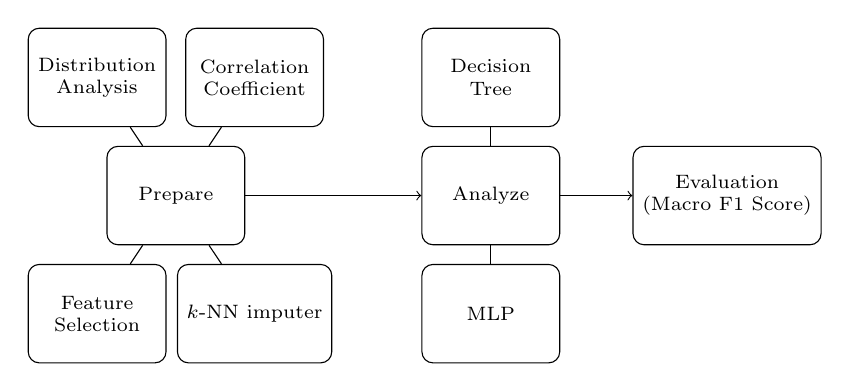
\begin{tikzpicture}[minimum width=1.75cm, minimum height=1.25cm, font=\scriptsize]
      \node[draw, align=center, rounded corners]  (P)   at ( 0,  0.0)    {Prepare};
      \node[draw, align=center, rounded corners]  (D)   at (-1,  1.5)    {Distribution \\ Analysis};
      \node[draw, align=center, rounded corners]  (C)   at ( 1,  1.5)    {Correlation \\ Coefficient};
      \node[draw, align=center, rounded corners]  (F)   at (-1, -1.5)    {Feature \\ Selection};
      \node[draw, align=center, rounded corners]  (KNN) at ( 1, -1.5)    {$k$-NN imputer};

      \node[draw, align=center, rounded corners]  (M)   at ( 4,  0.0)    {Analyze};
      \node[draw, align=center, rounded corners]  (DT)  at ( 4,  1.5)    {Decision \\ Tree};
      \node[draw, align=center, rounded corners]  (MLP) at ( 4, -1.5)    {MLP};

      \node[draw, align=center, rounded corners]  (E)   at ( 7,  0.0)    {Evaluation \\ (Macro F1 Score)};

      \draw[->] (P) -- (M);

      \draw[-]  (P) -- (D);
      \draw[-]  (P) -- (C);
      \draw[-]  (P) -- (F);
      \draw[-]  (P) -- (KNN);

      \draw[-]  (M) -- (DT);
      \draw[-]  (M) -- (MLP);

      \draw[->] (M) -- (E);
    \end{tikzpicture}
    \caption{Overview flowchart for task 2.}
  \end{figure}

\end{frame}

\begin{frame}{Task 2 - Data Distribution}

  \begin{table}[H]
    \centering
    \begin{tabular}{|c|c|c|c|c|c|}
      \hline
      Feature & \makecell{Number Of                               \\ Miss Value} & Feature & \makecell{Number Of \\ Miss Value} & Feature & \makecell{Number Of \\ Miss Value} \\
      \hline
      X01     & $0$                 & Y01 & $0$    & Z01 & $0$    \\
      \hline
      X11     & $0$                 & Y11 & $0$    & Z11 & $0$    \\
      \hline
      X21     & $0$                 & Y21 & $0$    & Z21 & $0$    \\
      \hline
      X31     & $355$               & Y31 & $355$  & Z31 & $355$  \\
      \hline
      X41     & $1604$              & Y41 & $1604$ & Z41 & $1604$ \\
      \hline
      X51     & $6634$              & Y51 & $6634$ & Z51 & $6634$ \\
      \hline
    \end{tabular}
    \caption{The number of missing values for each feature in training data. (The total number of data is $40000$.)}
  \end{table}

\end{frame}

\begin{frame}{Task 2 - Data Distribution}

  \begin{figure}[H]
    \centering
    \includegraphics[width=0.18\textwidth]{../code/Task2/Analysis/Hist-X01}
    \includegraphics[width=0.18\textwidth]{../code/Task2/Analysis/Hist-Y01}
    \includegraphics[width=0.18\textwidth]{../code/Task2/Analysis/Hist-Z01}
    \includegraphics[width=0.18\textwidth]{../code/Task2/Analysis/Hist-X11}
    \includegraphics[width=0.18\textwidth]{../code/Task2/Analysis/Hist-Y11} \\
    \includegraphics[width=0.18\textwidth]{../code/Task2/Analysis/Hist-Z11}
    \includegraphics[width=0.18\textwidth]{../code/Task2/Analysis/Hist-X21}
    \includegraphics[width=0.18\textwidth]{../code/Task2/Analysis/Hist-Y21}
    \includegraphics[width=0.18\textwidth]{../code/Task2/Analysis/Hist-Z21}
    \includegraphics[width=0.18\textwidth]{../code/Task2/Analysis/Hist-X31} \\
    \includegraphics[width=0.18\textwidth]{../code/Task2/Analysis/Hist-Y31}
    \includegraphics[width=0.18\textwidth]{../code/Task2/Analysis/Hist-Z31}
    \includegraphics[width=0.18\textwidth]{../code/Task2/Analysis/Hist-X41}
    \includegraphics[width=0.18\textwidth]{../code/Task2/Analysis/Hist-Y41}
    \includegraphics[width=0.18\textwidth]{../code/Task2/Analysis/Hist-Z41} \\
    \includegraphics[width=0.18\textwidth]{../code/Task2/Analysis/Hist-X51}
    \includegraphics[width=0.18\textwidth]{../code/Task2/Analysis/Hist-Y51}
    \includegraphics[width=0.18\textwidth]{../code/Task2/Analysis/Hist-Z51}
    \caption{The distribution for each feature (the top and bottom $5\%$ points are considered as outliers, and are not shown). The vertical lines shows the position of first, second and third quartiles.}
  \end{figure}

\end{frame}

\begin{frame}{Task 2 - Data Distribution}

  \begin{figure}[H]
    \centering
    \includegraphics[width=0.45\textwidth]{../code/Task2/Analysis/corrcoef-1.jpg}
    \includegraphics[width=0.45\textwidth]{../code/Task2/Analysis/corrcoef-2.jpg} \\
    \includegraphics[width=0.45\textwidth]{../code/Task2/Analysis/corrcoef-3.jpg}
    \includegraphics[width=0.45\textwidth]{../code/Task2/Analysis/corrcoef-4.jpg} \\
    \caption{Correlation coefficient for each features with label 1, 2, 3, 4.}
  \end{figure}

\end{frame}

\begin{frame}{Task 2 - Preformance - Decision Tree}

  \begin{table}[H]
    \centering
    \begin{tabular}{|c|c|c|c|c|c|}
      \hline
      \makecell{Max                                                  \\Depth} & \makecell{Num of                                                          \\ Threshold} & Criterion & \makecell{Feature \\ Selection}& \makecell{F1 Score \\ (Test/Train)} & \makecell{Time/Mem \\ (s/MB)}               \\
      \hline
      $10$ & $64$  & gini    & False & $0.8097/0.8359$ & $153.6/606$ \\
      \hline
      $10$ & $128$ & gini    & False & $0.8043/0.8512$ & $168.5/650$ \\
      \hline
      $12$ & $64$  & gini    & False & $0.8511/0.9106$ & $172.8/601$ \\
      \hline
      $10$ & $64$  & entropy & False & $0.8184/0.8596$ & $147.7/608$ \\
      \hline
      $10$ & $64$  & gini    & True  & $0.8052/0.8334$ & $80.7/585$  \\
      \hline
    \end{tabular}
    \caption{Preformance for decision tree. We tested each option with $5$ times cross validation ($80\%$ for training set, $20\%$ for training set) and $1$ times that using all data as training set. The f1 scores showed in the table is the average f1 score for cross validation and using all data as training set (in this case, we just tested the model on training data) and using all data as training set (in this case, we just tested the model on training data), the time is the total time for $6$ run, and the memory usage is tested using all the data as training set.}
  \end{table}

\end{frame}

\begin{frame}{Task 2 - Preformance - MLP}

  \begin{table}[H]
    \centering
    \begin{tabular}{|c|c|c|c|c|c|}
      \hline
      Dropout & \makecell{Hidden                                                \\ Size} & \makecell{Feature                                        \\ Selection} &\makecell{Batch \\ Size} & \makecell{F1 Score \\ (Test/Train)} & \makecell{Time/Mem \\ (s/MB)} \\
      \hline
      $0.3$   & $128$            & False & 512  & $0.9617/0.9718$ & $219.4/856$ \\
      \hline
      $0.3$   & $64$             & False & 512  & $0.9173/0.9253$ & $212.9/812$ \\
      \hline
      $0.3$   & $256$            & False & 512  & $0.9767/0.9939$ & $221.7/856$ \\
      \hline
      $0.3$   & $128$            & False & 1024 & $0.9629/0.9743$ & $148.6/857$ \\
      \hline
      $0.3$   & $128$            & False & 512  & $0.9644/0.9750$ & $381.4/859$ \\
      \hline
      $0.3$   & $128$            & True  & 512  & $0.9474/0.9559$ & $171.7/848$ \\
      \hline
    \end{tabular}
    \caption{Preformance for MLP. We tested each option with $5$ times cross validation ($80\%$ for training set, $20\%$ for training set) and $1$ times that using all data as training set. The f1 scores showed in the table is the average f1 score for cross validation and using all data as training set (in this case, we just tested the model on training data), the time is the total time for $6$ run, and the memory usage is tested using all the data as training set.}
  \end{table}

\end{frame}

\subsection{Solution - Task 3}

\begin{frame}{Task 3 - Overview}

  \begin{figure}[H]
    \centering
    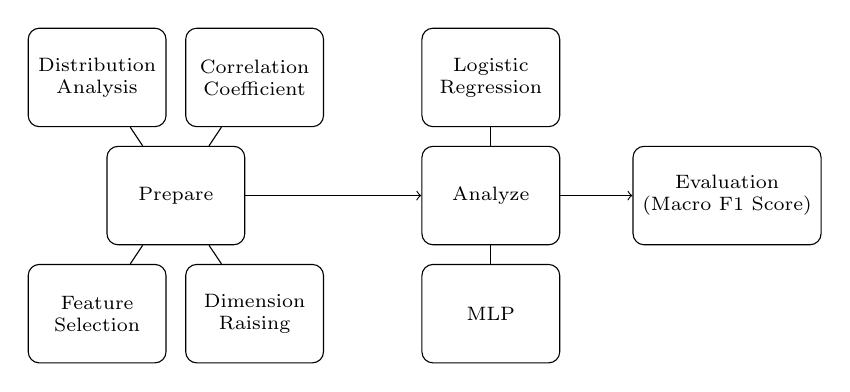
\begin{tikzpicture}[minimum width=1.75cm, minimum height=1.25cm, font=\scriptsize]
      \node[draw, align=center, rounded corners]  (P)   at ( 0,  0.0)    {Prepare};
      \node[draw, align=center, rounded corners]  (D)   at (-1,  1.5)    {Distribution \\ Analysis};
      \node[draw, align=center, rounded corners]  (C)   at ( 1,  1.5)    {Correlation \\ Coefficient};
      \node[draw, align=center, rounded corners]  (F)   at (-1, -1.5)    {Feature \\ Selection};
      \node[draw, align=center, rounded corners]  (R)   at ( 1, -1.5)    {Dimension \\ Raising};

      \node[draw, align=center, rounded corners]  (M)   at ( 4,  0.0)    {Analyze};
      \node[draw, align=center, rounded corners]  (LR)  at ( 4,  1.5)    {Logistic \\ Regression};
      \node[draw, align=center, rounded corners]  (MLP) at ( 4, -1.5)    {MLP};

      \node[draw, align=center, rounded corners]  (E)   at ( 7,  0.0)    {Evaluation \\ (Macro F1 Score)};

      \draw[->] (P) -- (M);

      \draw[-]  (P) -- (D);
      \draw[-]  (P) -- (C);
      \draw[-]  (P) -- (F);
      \draw[-]  (P) -- (R);

      \draw[-]  (M) -- (LR);
      \draw[-]  (M) -- (MLP);

      \draw[->] (M) -- (E);
    \end{tikzpicture}
    \caption{Overview flowchart for task 3.}
  \end{figure}

\end{frame}

\begin{frame}{Task 3 - Distribution Analysis}

  \begin{figure}[H]
    \centering
    \includegraphics[width=\textwidth]{../code/Task3/Analysis/PC.jpg}
    \caption{The parallel coordinate plot for each features (we chose $10\%$ of total data).}
  \end{figure}

\end{frame}

\begin{frame}{Task 3 - Distribution Analysis}

  \begin{figure}[H]
    \centering
    \includegraphics[width=\textwidth]{../code/Task3/Analysis/corrcoef.jpg} \\
    \caption{Correlation coefficient for each features.}
  \end{figure}

\end{frame}

\begin{frame}{Task 3 - Preformance - Logistic Regression}

  \begin{table}[H]
    \centering
    \begin{tabular}{|c|c|c|c|c|}
      \hline
      Penalty & \makecell{Dimension                                        \\ Raising \\ (Degree)} & \makecell{Feature \\ Selection} & \makecell{F1 Score \\ (Test/Train)} & \makecell{Time/Mem \\ (s/MB)} \\
      \hline
      None    & None                & False & $0.9586/0.9577$ & $19.5/866$ \\
      \hline
      None    & $2$                 & False & $0.9619/0.9610$ & $33.5/915$ \\
      \hline
      None    & $3$                 & False & $0.9621/0.9612$ & $49.6/973$ \\
      \hline
      Lasso   & None                & False & $0.9579/0.9570$ & $21.5/854$ \\
      \hline
      Ridge   & None                & False & $0.9553/0.9544$ & $19.8/853$ \\
      \hline
      None    & None                & True  & $0.9582/0.9573$ & $16.5/825$ \\
      \hline
    \end{tabular}
    \caption{Preformance for logistic regression. We tested each option with $5$ times cross validation ($80\%$ for training set, $20\%$ for training set) and $1$ times that using all data as training set. The f1 scores showed in the table is the average f1 score for cross validation and using all data as training set (in this case, we just tested the model on training data), the time is the total time for $6$ run, and the memory usage is tested using all the data as training set.}
  \end{table}

\end{frame}

\begin{frame}{Task 3 - Preformance - MLP}

  \begin{table}[H]
    \centering
    \begin{tabular}{|c|c|c|c|c|}
      \hline
      Dropout & Hidden Size & \makecell{Feature                                \\ Selection} & \makecell{F1 Score \\ (Test/Train)} & \makecell{Time/Mem \\ (s/MB)} \\
      \hline
      $0.1$   & $32$        & False             & $0.9522/0.9548$ & $31.9/929$ \\
      \hline
      $0.2$   & $32$        & False             & $0.9000/0.9207$ & $31.1/916$ \\
      \hline
      $0.1$   & $32$        & True              & $0.9481/0.9480$ & $31.3/899$ \\
      \hline
      $0.1$   & $16$        & False             & $0.9503/0.9493$ & $31.7/929$ \\
      \hline
      $0.1$   & $64$        & True              & $0.9500/0.9501$ & $29.7/902$ \\
      \hline
    \end{tabular}
    \caption{Preformance for MLP. We tested each option with $5$ times cross validation ($80\%$ for training set, $20\%$ for training set) and $1$ times that using all data as training set. The f1 scores showed in the table is the average f1 score for cross validation and using all data as training set (in this case, we just tested the model on training data), the time is the total time for $6$ run, and the memory usage is tested using all the data as training set.}
  \end{table}

\end{frame}

\section{Summary}

\begin{frame}{Summary}

\end{frame}

\section*{Reference}
\begin{frame}[allowframebreaks]{Reference}
  \printbibliography
\end{frame}

\appendix

\end{document}